% Section content template for individual Educative lessons
% This file contains the actual content for a specific section
% Generated from Educative API section content

% Section: Requirements of a Rate Limiter’s Design
% Section ID: 5887506125422592
% Section Slug: requirements-of-a-rate-limiters-design
% Generated: 2025-12-07T21:29:04.151919

\subsection{Requirements}\label{5iIMoFidxXrrvxkxGeMYq}
\\
Our focus in this lesson is to design a rate limiter with the following functional and non-functional requirements.

\subsubsection{Functional requirements}\label{NTyGAt68lfKAjDqwXYkZA}

\begin{itemize}
\item
\protect\phantomsection\label{lHw9OwEqGwsrAh4ra4_kp}
To limit the number of requests a client can send to an API within a time window.
\item
\protect\phantomsection\label{CJKVWv_eCd8tGacJZIJ-3}
To make the limit of requests per window configurable.
\item
\protect\phantomsection\label{knzH90E0RnYqegHqO_h3Y}
To make sure that the client gets a message (error or notification) whenever the defined threshold is crossed within a single server or combination of servers.
\end{itemize}

\subsubsection{Non-functional requirements}\label{wxFOM0BwLtwbwGFQKQpqv}

\begin{itemize}
\item
\protect\phantomsection\label{JdEMZBzSxBHee43v-XECd}
\textbf{Availability:} Essentially, the rate limiter protects our system. Therefore, it should be highly available.
\item
\protect\phantomsection\label{nNaVz3wJLrOpMte3jvoyu}
\textbf{Low latency:} Because all API requests pass through the rate limiter, it should work with a minimum latency without affecting the user experience.
\item
\protect\phantomsection\label{Vmj8DSaWJsOIb-fWGVlxg}
\textbf{Scalability:} Our design should be highly scalable. It should be able to rate limit an increasing number of clients' requests over time.
\end{itemize}

\subsection{Types of throttling}\label{jy4TfMoOPypaf23FydLHO}
\\
A rate limiter can perform three types of throttling.

\begin{enumerate}
\item
\protect\phantomsection\label{fV7AuMqpJwamMqDU-fs9i}
\textbf{Hard throttling:} This type of throttling puts a hard limit on the number of API requests. So, whenever a request exceeds the limit, it is discarded.
\item
\protect\phantomsection\label{Ox-xO-LyJbr65VOLJhPwB}
\textbf{Soft throttling:} Under soft throttling, the number of requests can exceed the predefined limit by a certain percentage. For example, if our system has a predefined limit of 500 messages per minute with a 5\% exceed in the limit, we can let the client send 525 requests per minute.
\item
\protect\phantomsection\label{xUKIb35mYeh_VXF7kj_Jc}
\textbf{Elastic or dynamic throttling:} In this throttling, the number of requests can cross the predefined limit if the system has excess resources available. However, there is no specific percentage defined for the upper limit. For example, if our system allows 500 requests per minute, it can let the user send more than 500 requests when free resources are available.
\end{enumerate}

Linux operating systems provide a kernel feature known as \texttt{cgroups} (control groups) that limits, accounts for, and isolates the resources---CPU time, system memory, disk storage, I/O, and network bandwidth---of a collection of processes. By using \texttt{cgroups}, the system administrator can monitor, deny access to specific resources, and reconfigure the \texttt{cgroups} dynamically on a running system. The
\texttt{cgroups} feature provides the following benefits through which the system administrator gains a fine-grain control of the system resources:

\begin{itemize}
\item
\textbf{Resource limiting:} Using this feature, a restriction can be imposed on groups not to exceed a configured memory limit and file system cache.
\item
\textbf{Prioritization:} Through this feature, some groups can be prioritized to use a larger share of CPU cycles or disk I/O throughput.
\item
\textbf{Accounting:} This feature is used to measure a group's resource usage, which could also be used for billing purposes.
\item
\textbf{Control:} The system administrator can control groups of processes, their checkpoints, and restart via this feature.
\end{itemize}
\\
Providing such rich features, \texttt{cgroup} can be used at a system (single server) level to limit resource usage not only for a single user but also for groups of users or processes.
\\
We can extend the above concepts by designing a service that takes input from the rate-limiting service and enforces the limits on local nodes of a cluster.

\subsection{Where to place the rate limiter}\label{S2iplHP53y2tGnZrs-wC8}
\\
There are three different ways to place the rate limiter.

\begin{enumerate}
\item
\protect\phantomsection\label{UwRV1VcYEwWnnJ1NqoYdk}
\textbf{On the client side:} It is easy to place the rate limiter on the client side. However, this strategy is not safe because it can easily be tampered with by malicious activity. Moreover, the configuration on the client side is also difficult to apply in this approach.
\item
\protect\phantomsection\label{mxXOGPuhQ-Alwji8qiwkR}
\textbf{On the server side:} As shown in the following figure, the rate limiter is placed on the server-side. In this approach, a server receives a request that is passed through the rate limiter that resides on the server.
\end{enumerate}

\begin{figure}[htbp]
 \centering
 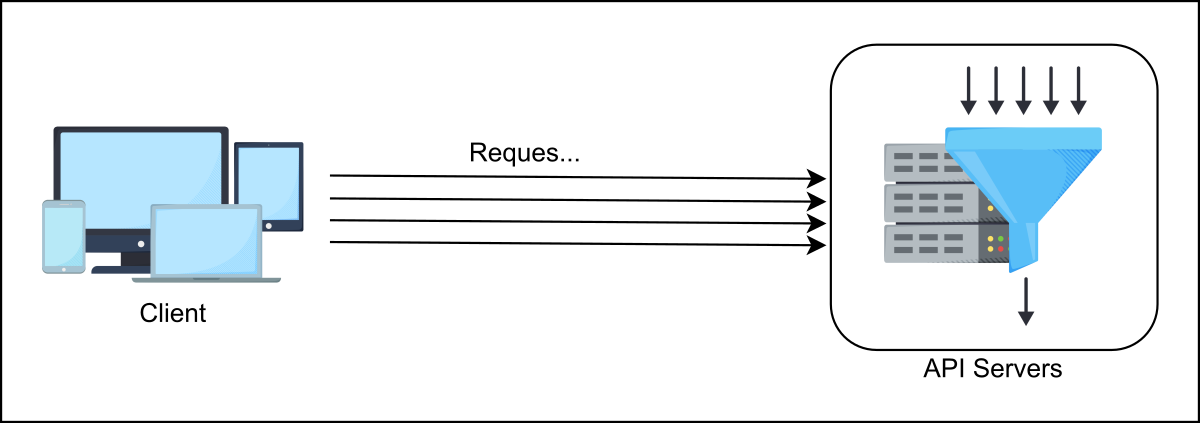
\includegraphics[width=0.5\textwidth]{Images/chapter_19/section_5887506125422592/6733040598777856.png}
 \caption{Rate limiter placed at the server side}
\end{figure}

\begin{enumerate}
\setcounter{enumi}{2}
\item
\protect\phantomsection\label{O9z5bN3njWkifvrKcxsJj}
\textbf{As middleware:} In this strategy, the rate limiter acts as middleware, throttling requests to API servers as shown in the following figure.
\end{enumerate}

\begin{figure}[htbp]
 \centering
 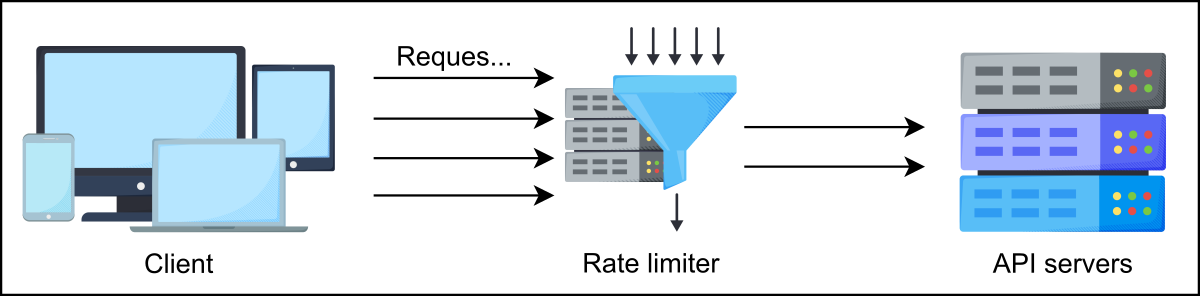
\includegraphics[width=0.5\textwidth]{Images/chapter_19/section_5887506125422592/4623965350133760.png}
 \caption{Rate limiter as middleware}
\end{figure}

Placing a rate limiter is dependent on a number of factors and is a subjective decision, based on the organization's technology stack, engineering resources, priorities, plan, goals, and so on.
\begin{quote}
\textbf{Note:} Many modern services use APIs to provide their functionality to the clients. API endpoints can be a good vantage point to rate limit the incoming client traffic because all traffic passes through them.
\end{quote}
\subsection{Two models for implementing a rate limiter}\label{l5XczAjX5CVl3aNiVAz69}
\\
One rate limiter might not be enough to handle enormous traffic to support millions of users. Therefore, a better option is to use multiple rate limiters as a cluster of independent nodes. Since there will be numerous rate limiters with their corresponding counters (or their rate limit), there are two ways to use databases to store, retrieve, and update the counters along with the user information.

\begin{enumerate}
\item
\protect\phantomsection\label{EXY1Hd2d7V_gAWs-PN-mZ}
\textbf{A rate limiter with a centralized database:} In this approach, rate limiters interact with a centralized database, preferably Redis or PostgreSQL. The advantage of this model is that the counters are stored in centralized databases. Therefore, a client can't exceed the predefined limit. However, there are a few drawbacks to this approach. It causes an increase in latency if an enormous number of requests hit the centralized database. Another extensive problem is the potential for race conditions in highly concurrent requests (or associated lock contention).
\item
\protect\phantomsection\label{TkBoBDGUoFy-UK3hWT0xS}
\textbf{A rate limiter with a distributed database:} Using an independent cluster of nodes is another approach where the rate-limiting state is in a distributed database. In this approach, each node has to track the rate limit. The problem with this approach is that a client could exceed a rate limit---at least momentarily, while the state is being collected from everyone---when sending requests to different nodes (rate-limiters). To enforce the limit, we must set up sticky sessions in the load balancer to send each consumer to exactly one node. However, this approach lacks fault tolerance and poses scaling problems when the nodes get overloaded.
\end{enumerate}
\\
Aside from the above two concepts, another problem is whether to use a global counter shared by all the incoming requests or individual counters per user. For example, the \href{https://www.educative.io/courses/grokking-the-system-design-interview/rate-limiter-algorithms\#Token-bucket-algorithm}{token bucket algorithm} can be implemented in two ways. In the first method, all requests can share the total number of tokens in a single bucket, while in the second method, individual buckets are assigned to users. The choice of using shared or separate counters (or buckets) depends on the use case and the rate-limiting rules.

\begin{quote}
\textbf{Quiz:}
\textbf{Question 1:} Can a load balancer be used as a rate limiter?
\textbf{Answer:} Load balancers play a critical role in preventing an application server from being overwhelmed by an excessive number of requests. They achieve this by either declining requests based on predefined limits or directing them to a queue for deferred processing. It's essential to emphasize that load balancers treat all incoming requests impartially,

without recognizing the diverse complexities and processing durations associated with different operations. For instance, certain operations within a web service may be rapid, while others may be more time-intensive. When there is a need to control the number of requests for specific operations, a more effective approach is to implement this control at the application server level using a rate limiter. The rate limiter excels at understanding the intricacies of individual operations and can selectively impose limitations as required.
\textbf{Question 2:} Assume a scenario in which a client intends to send requests for a particular service using two virtual machines (VMs), where one is using a VPN to a different region. Suppose that the throttling identifier works based on user credentials. Therefore, the user ID would be the same for both sessions. Moreover, let's assume that requests from different VMs can hit different data centers. How would the throttling work to prevent the user from exceeding the rate limit in this scenario?
\textbf{Answer:} To rate limit the incoming requests, we have two different choices to place the rate limiter. 1. Rate limiter per data center: One way to throttle the incoming requests from the user is to use rate limiting per data centers. Each data center will have its own rate-limiter, which limits the incoming requests. In this approach, the rate (count or rate limit) is relatively lower. Therefore, a limited number of requests are allowed per unit time. Moreover, this approach provides lower latency since the requests are normally directed to the nearest data centers located geographically. Often, latency within a data center is less than one millisecond and multiple redundant paths are available in case of some link failure. 2. A shared rate limiter across data centers:

Another approach is to use a shared rate limiter across multiple data centers. This way, requests received from both VMs will be throttled by the single rate limiter. The number of requests allowed in this case is higher. However, this approach is relatively slower, as prior to directing a request to any nearest data center, it will pass through the shared rate limiter. Latency is often high and variable across geographically distributed data centers and not a lot of redundant paths are available. If rate limiting is applied independently per data center without global coordination, users could potentially exceed the limit by distributing requests across multiple data centers. To prevent this, a globally shared rate limiter (e.g., a distributed token bucket) would be needed to enforce a consistent limit across all data centers.
\end{quote}

\subsection{Building blocks we will use}\label{3IXftg5uZSmX4QjkBYiv7}
\\
The design of the rate limiter utilizes the following building blocks that we discussed in the initial chapters.\\

\begin{figure}[htbp]
 \centering
 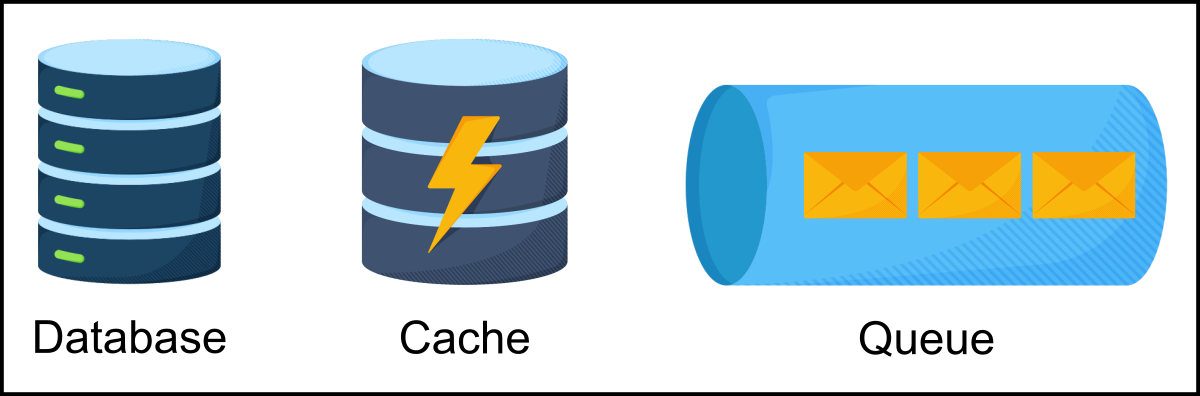
\includegraphics[width=0.5\textwidth]{Images/chapter_19/section_5887506125422592/6252760360419328.png}
 \caption{Building blocks in the design of a rate limiter}
\end{figure}

\begin{itemize}
\item
\protect\phantomsection\label{ZGXG_Qog_h3OMnhk3hD3_}
\href{https://www.educative.io/courses/grokking-the-system-design-interview/introduction-to-databases}{\textbf{Databases}} are used to store rules defined by a service provider and metadata of users using the service.
\item
\protect\phantomsection\label{swzwQHDodggiKB4X-AZCR}
\href{https://www.educative.io/courses/grokking-the-system-design-interview/system-design-the-distributed-cache}{\textbf{Caches}} are used to cache the rules and users' data for frequent access.
\item
\protect\phantomsection\label{ew2o2AvUSnA8BE60aB-5_}
\href{https://www.educative.io/courses/grokking-the-system-design-interview/requirements-of-a-distributed-messaging-queues-design}{\textbf{Queues}} are essential for holding the incoming requests that are allowed by the rate limiter.
\end{itemize}
\\
In the next lesson, we'll focus on a high-level and detailed design of a rate limiter based on the requirements discussed in this lesson.

% End of section content